\documentclass{beamer}
\usetheme{Boadilla}
\usepackage{booktabs}
\usepackage{adjustbox}
\usefonttheme{serif}
\subtitle{Using Beamer}
\usepackage{pgffor}
\usepackage{graphicx}
\usepackage{booktabs}




\title{ \textbf{Stepscan Project}}
\subtitle{Results of Worksheet 1-3}
\date{\today}
\author{Saeed Kazemi}
\institute{ University of New Brunswick}
\usepackage{caption}

\begin{document}


%%%%%%%%%%%%%%%%%%%%%%%%%%%%%%%%%%%%%%%%%%%
%%%%%%%%%%%%%%%%%%%%%%%%%%%%%%%%%%%%%%%%%%%
\begin{frame}
\titlepage
\end{frame}


%%%%%%%%%%%%%%%%%%%%%%%%%%%%%%%%%%%%%%%%%%%
%%%%%%%%%%%%%%%%%%%%%%%%%%%%%%%%%%%%%%%%%%%
\begin{frame}
\frametitle{Outline}
\tableofcontents
\end{frame}


%%%%%%%%%%%%%%%%%%%%%%%%%%%%%%%%%%%%%%%%%%%
%%%%%%%%%%%%%%%%%%%%%%%%%%%%%%%%%%%%%%%%%%%
\iffalse

\section{Test Size}
    \begin{frame}
    \frametitle{Comparing different test size over Pressure Features}
    \tiny
    \begin{table}
    \centering
    \captionsetup{labelformat=empty}
    \caption{\footnotesize Comparing Accuracy and EER of different test size over Pressure Features. These results are average of both sides.}
    \begin{tabular}{llll}
\toprule
{} &                        Accuracy &                        F1-score &                         EER \\
\midrule
0.10 &  69.89 +/- 33.78 (64.35, 75.85) &  64.47 +/- 29.38 (57.27, 72.84) &  0.30 +/- 0.14 (0.24, 0.36) \\
0.20 &  69.18 +/- 33.68 (64.51, 75.06) &  66.61 +/- 31.16 (59.18, 74.39) &  0.31 +/- 0.15 (0.25, 0.35) \\
0.25 &  69.45 +/- 33.76 (64.74, 75.27) &  67.65 +/- 32.25 (61.43, 74.88) &  0.31 +/- 0.14 (0.25, 0.35) \\
0.30 &  69.54 +/- 33.73 (65.24, 75.04) &  67.95 +/- 32.08 (62.13, 75.01) &  0.30 +/- 0.14 (0.25, 0.35) \\
0.40 &  67.87 +/- 32.88 (63.23, 72.88) &  65.85 +/- 31.35 (60.21, 72.06) &  0.32 +/- 0.15 (0.27, 0.37) \\
0.50 &  67.11 +/- 33.10 (62.08, 72.49) &  65.00 +/- 31.63 (58.09, 72.04) &  0.33 +/- 0.16 (0.28, 0.38) \\
0.60 &  66.11 +/- 32.43 (61.15, 71.35) &  63.61 +/- 30.34 (56.10, 71.12) &  0.34 +/- 0.16 (0.29, 0.39) \\
0.70 &  64.59 +/- 31.92 (60.42, 69.34) &  60.23 +/- 29.49 (53.17, 68.38) &  0.35 +/- 0.17 (0.31, 0.40) \\
0.75 &  61.88 +/- 31.08 (58.57, 66.35) &  55.02 +/- 27.49 (45.77, 64.80) &  0.38 +/- 0.19 (0.34, 0.41) \\
0.80 &  60.31 +/- 30.40 (57.32, 64.33) &  51.32 +/- 25.46 (39.65, 61.67) &  0.40 +/- 0.19 (0.36, 0.43) \\
0.90 &  54.94 +/- 27.89 (53.20, 57.76) &  33.49 +/- 17.25 (10.93, 64.48) &  0.45 +/- 0.22 (0.42, 0.47) \\
\bottomrule
\end{tabular}

    \end{table}
    
    \begin{block}{\footnotesize Conditions}
        \tiny These results are average over the results of below conditions:
        \begin{itemize} 
            \item min, mean and median criteria,
            \item Both correlation and distance score matrix
            \item Keeping 95\% variances
            \item Z-score algorithm
        \end{itemize} 
    \end{block}
    
    \end{frame}
    
    
    
    \begin{frame}
    \centering
    \frametitle{Comparing different test size over Pressure Features}
    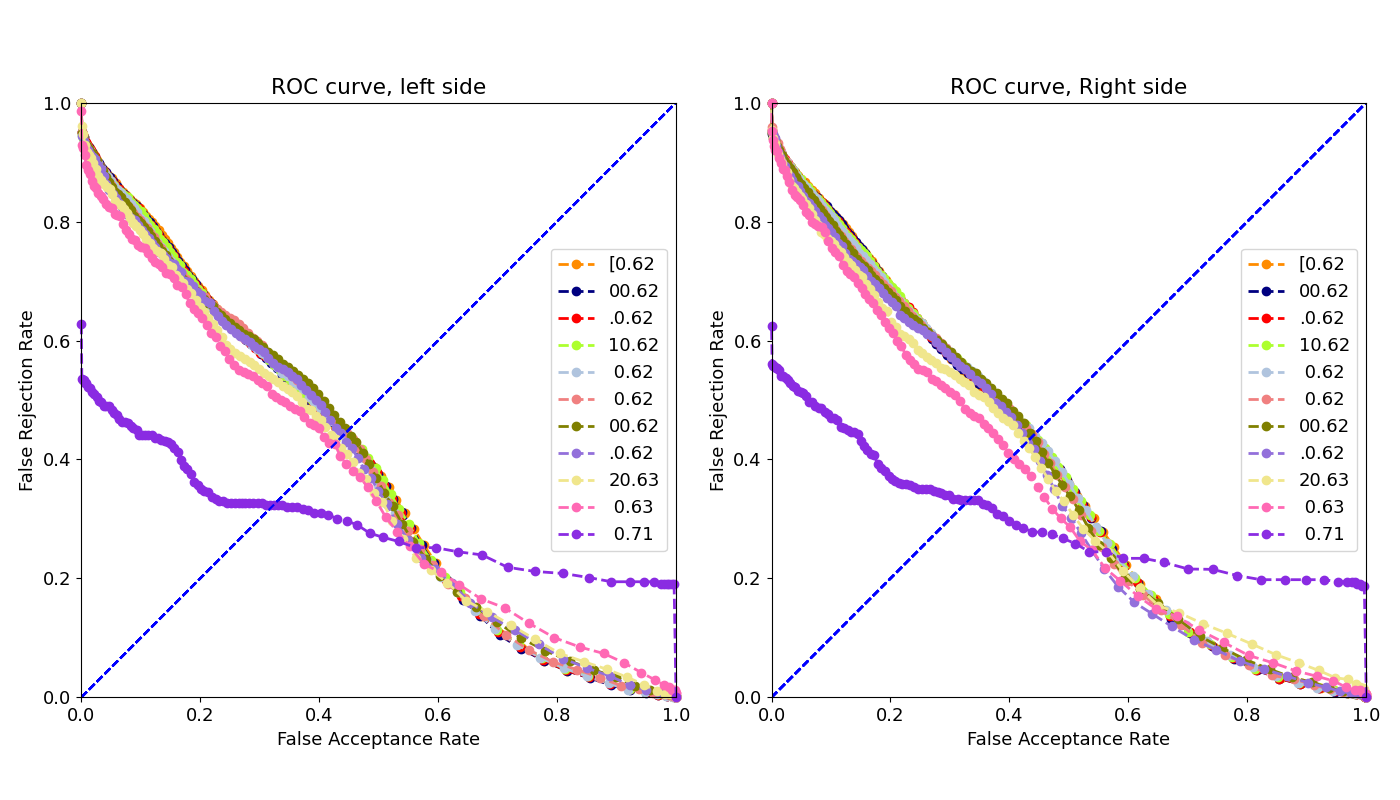
\includegraphics[scale=0.3]{Manuscripts/src/figures/testsize.png}
    \end{frame}

    
    

\fi

\section{Score Matrix}
    \foreach \n in {afeatures-simple, afeatures-otsu, pfeatures, COAs-otsu, COAs-simple, COPs}{
    \begin{frame}
    \frametitle{Euclidean distance vs Correlation over \n}
    \tiny
    \begin{table}
    \centering
    \captionsetup{labelformat=empty}
    \caption{\footnotesize The accuracy of Euclidean distance and Correlation on \n.}
    \input{Manuscripts/src/tables/\n-Mode-Acc}
    \end{table}
    \begin{table}
    \centering
    \captionsetup{labelformat=empty}
    \caption{\footnotesize The EER of Euclidean distance and Correlation on \n}
    \label{tab:parameters condition}
    \input{Manuscripts/src/tables/\n-Mode-EER}
    \end{table}
    
    \begin{block}{\footnotesize Conditions}
        \tiny These results are average over the results of below conditions: min, mean and median criteria, All PCs and 95\% variances, Min-Max and z-score algorithm. also all features in \n \ were considered.
    \end{block}
    
    \end{frame}
    
    
    
    \begin{frame}
    \centering
    \frametitle{Euclidean distance vs Correlation (ROC curve) over \n}
    \includegraphics[scale=0.3]{Manuscripts/src/figures/\n-Mode.png}
    \end{frame}
    
    }

%%%%%%%%%%%%%%%%%%%%%%%%%%%%%%%%%%%%%%%%%%%
%%%%%%%%%%%%%%%%%%%%%%%%%%%%%%%%%%%%%%%%%%%
\section{PCA}
    \foreach \n in {afeatures-simple, afeatures-otsu, pfeatures, COAs-otsu, COAs-simple, COPs}{
    \begin{frame}
    \frametitle{All PCs vs 95\% variance over \n}
    \tiny
    \begin{table}
    \centering
    \captionsetup{labelformat=empty}
    \caption{\footnotesize The accuracy of All PCs and 95\% variance over \n}
    \input{Manuscripts/src/tables/\n-PCA-Acc}
    \end{table}
    \begin{table}
    \centering
    \captionsetup{labelformat=empty}
    \caption{\footnotesize The EER of All PCs and 95\% variance over \n}
    \label{tab:parameters condition}
    \input{Manuscripts/src/tables/\n-PCA-EER}
    \end{table}
    
    \begin{block}{\footnotesize Conditions}
        \tiny These results are average over the results of below conditions: min, mean and median criteria, correlation and distant score, Min-Max and z-score algorithm. also all features in \n \ were considered.
    \end{block}
    
    \end{frame}
    
    
    
    \begin{frame}
    \centering
    \frametitle{All PCs vs 95\% variance over \n}
    \includegraphics[scale=0.3]{Manuscripts/src/figures/\n-PCA.png}
    \end{frame}
    
    }
\section{Normalization algorithm}
    \foreach \n in {afeatures-simple, afeatures-otsu, pfeatures, COAs-otsu, COAs-simple, COPs}{
    \begin{frame}
    \frametitle{Min-Max vs z-score over \n}
    \tiny
    \begin{table}
    \centering
    \captionsetup{labelformat=empty}
    \caption{\footnotesize The accuracy of Min-Max and z-score algorithm over \n}
    \input{Manuscripts/src/tables/\n-Normalizition-Acc}
    \end{table}
    \begin{table}
    \centering
    \captionsetup{labelformat=empty}
    \caption{\footnotesize The EER of Min-Max and z-score algorithm over \n}
    \label{tab:parameters condition}
    \input{Manuscripts/src/tables/\n-Normalizition-EER}
    \end{table}
    
    \begin{block}{\footnotesize Conditions}
        \tiny These results are average over the results of below conditions: min, mean and median criteria, correlation and distant score, All PCs and 95\% variances. also all features in \n \ were considered.
    \end{block}
    
    \end{frame}
    
    
    
    \begin{frame}
    \centering
    \frametitle{Min-Max vs z-score over \n}
    \includegraphics[scale=0.3]{Manuscripts/src/figures/\n-Normalizition.png}
    \end{frame}
    
    }
\section{Criteria}
    \foreach \n in {afeatures-simple, afeatures-otsu, pfeatures, COAs-otsu, COAs-simple, COPs}{
    \begin{frame}
    \frametitle{Comparing different criteria over \n}
    \tiny
    \begin{table}
    \centering
    \captionsetup{labelformat=empty}
    \caption{\footnotesize The accuracy of The EER of min, mean and median criteria over \n}
    \input{Manuscripts/src/tables/\n-Model-Type-Acc}
    \end{table}
    \begin{table}
    \centering
    \captionsetup{labelformat=empty}
    \caption{\footnotesize The EER of min, mean and median criteria over \n}
    \label{tab:parameters condition}
    \input{Manuscripts/src/tables/\n-Model-Type-EER}
    \end{table}
    
    \begin{block}{\footnotesize Conditions}
        \tiny These results are average over the results of below conditions: correlation and distant score, All PCs and 95\% variances and Min-max and z-score algorithm. also all features in \n \ were considered.
    \end{block}
    
    \end{frame}
    
    
    
    \begin{frame}
    \centering
    \frametitle{Comparing different criteria over \n}
    \includegraphics[scale=0.3]{Manuscripts/src/figures/\n-Model-Type.png}
    \end{frame}
    
    }
\section{Features}
    \foreach \n in {afeatures-simple, afeatures-otsu, pfeatures, COX-time-series}{
    \begin{frame}
    \frametitle{Comparing different extracted features over \n}
    \tiny
    \begin{table}
    \centering
    \captionsetup{labelformat=empty}
    \caption{\footnotesize The accuracy of different extracted features over \n}
    \input{Manuscripts/src/tables/\n-Acc}
    \end{table}
    
    
    \begin{block}{\footnotesize Conditions}
        \tiny These results are average over the results of below conditions: min, mean and median criteria, correlation and distant score, All PCs and 95\% variances and Min-max and z-score algorithm.
    \end{block}
    
    \end{frame}
    
    \begin{frame}
    \frametitle{Comparing different extracted features over \n}
    \tiny
    \begin{table}
    \centering
    \captionsetup{labelformat=empty}
    \caption{\footnotesize The EER of different extracted features over \n}
    \label{tab:parameters condition}
    \input{Manuscripts/src/tables/\n-EER}
    \end{table}
    
    \begin{block}{\footnotesize Conditions}
        \tiny These results are average over the results of below conditions: min, mean and median criteria, correlation and distant score, All PCs and 95\% variances and Min-max and z-score algorithm.
    \end{block}
    
    \end{frame}
    
    \begin{frame}
    \centering
    \frametitle{Comparing different extracted features over \n}
    \includegraphics[scale=0.3]{Manuscripts/src/figures/\n.png}
    \end{frame}
    
    }
\section{Features selection}
    \foreach \n in {afeatures-simple, afeatures-otsu, pfeatures}{
    \begin{frame}
    \frametitle{Comparing different extracted features over \n \ based on FS algorithm}
    \tiny
    \begin{table}
    \centering
    \captionsetup{labelformat=empty}
    \caption{\footnotesize The top 10 features over \n}
    \input{Manuscripts/src/tables/\n-10best-FS}
    \end{table}
    
    
  
    
    \end{frame}
    
    \begin{frame}
    \frametitle{Comparing different extracted features over \n \ based on FS algorithm}
    \tiny
    \begin{table}
    \centering
    \captionsetup{labelformat=empty}
    \caption{\footnotesize The top 10 features over \n}
    \label{tab:parameters condition}
    \input{Manuscripts/src/tables/\n-10worst-FS}
    \end{table}
    
    \end{frame}
    

    
    }
\section{The best and worst top models}
    \begin{frame}[shrink = 35]
    \frametitle{The best top models}
    \tiny
    \begin{table}
    \centering
    \captionsetup{labelformat=empty}
    \caption{\footnotesize The top 10 models on left foot.}
    \begin{tabular}{llllrllrlrrrr}
\toprule
{} &      Feature\_Type &  Mode & Criteria &  Test\_Size & Normalizition & Features\_Set &  PCA & template-selection-method &  k-cluster &  Mean\_Acc\_L &  Mean\_f1\_L &  Mean\_EER\_L\_tr \\
\midrule
0 &         pfeatures &  dist &      ave &        0.3 &       z-score &        RANGE &  1.0 &                      None &          4 &       73.58 &      73.89 &           0.63 \\
0 &         pfeatures &  dist &      min &        0.3 &       z-score &        RANGE &  1.0 &                      None &          4 &       73.38 &      73.79 &           0.62 \\
0 &         pfeatures &  dist &      min &        0.3 &       z-score &        RANGE &  1.0 &                     MDIST &         12 &       73.26 &      73.06 &           0.62 \\
0 &         pfeatures &  dist &      ave &        0.3 &       z-score &        RANGE &  1.0 &                     MDIST &         12 &       72.99 &      72.27 &           0.63 \\
0 &    afeatures-otsu &  dist &      ave &        0.3 &       z-score &        RANGE &  1.0 &                      None &          4 &       72.61 &      73.03 &           0.63 \\
0 &  afeatures-simple &  dist &      ave &        0.3 &       z-score &        RANGE &  1.0 &                      None &          4 &       72.32 &      71.32 &           0.63 \\
0 &    afeatures-otsu &  dist &      ave &        0.3 &       z-score &        RANGE &  1.0 &                     MDIST &         12 &       71.99 &      71.18 &           0.64 \\
0 &         pfeatures &  dist &      med &        0.3 &       z-score &        RANGE &  1.0 &                      None &          4 &       71.57 &      69.65 &           0.64 \\
0 &         pfeatures &  dist &      min &        0.3 &       z-score &        RANGE &  1.0 &                      DEND &          4 &       71.42 &      75.72 &           0.61 \\
0 &  afeatures-simple &  dist &      ave &        0.3 &       z-score &        RANGE &  1.0 &                     MDIST &         12 &       71.40 &      69.59 &           0.63 \\
\bottomrule
\end{tabular}

    \end{table}
    
    
    \begin{table}
    \centering
    \captionsetup{labelformat=empty}
    \caption{\footnotesize The top 10 models on right foot.}
    \begin{tabular}{llllrlllrrr}
\toprule
{} &      Feature\_Type &                Mode & Model-Type &  Test\_Size &      Normalizition & Features\_Set &      PCA &  Mean\_Acc\_R &  Mean\_f1\_R &  Mean\_EER\_R \\
\midrule
0 &  afeatures-simple &  Euclidean distance &    average &        0.2 &  Z-score algorithm &        RANGE &  All PCs &       72.71 &      71.93 &        0.29 \\
0 &         pfeatures &  Euclidean distance &    average &        0.2 &  Z-score algorithm &        RANGE &  All PCs &       72.61 &      71.88 &        0.29 \\
0 &         pfeatures &  Euclidean distance &    average &        0.2 &  Z-score algorithm &        TOTEX &  All PCs &       72.14 &      72.43 &        0.31 \\
0 &    afeatures-otsu &  Euclidean distance &    average &        0.2 &  Z-score algorithm &        RANGE &  All PCs &       72.11 &      70.39 &        0.30 \\
0 &  afeatures-simple &  Euclidean distance &        min &        0.2 &  Z-score algorithm &        TOTEX &  All PCs &       71.77 &      71.09 &        0.31 \\
0 &         pfeatures &  Euclidean distance &    average &        0.2 &  Z-score algorithm &        MVELO &  All PCs &       71.68 &      72.19 &        0.31 \\
0 &  afeatures-simple &  Euclidean distance &        min &        0.2 &  Z-score algorithm &        MVELO &  All PCs &       71.25 &      70.79 &        0.31 \\
0 &         pfeatures &  Euclidean distance &     median &        0.2 &  Z-score algorithm &        RANGE &  All PCs &       71.20 &      68.73 &        0.28 \\
0 &         pfeatures &  Euclidean distance &    average &        0.2 &   Minmax algorithm &        RANGE &  All PCs &       71.11 &      69.55 &        0.32 \\
0 &  afeatures-simple &  Euclidean distance &        min &        0.2 &   Minmax algorithm &        MVELO &  All PCs &       71.07 &      70.08 &        0.32 \\
\bottomrule
\end{tabular}

    \end{table}
    
    
    \end{frame}
    

    
    
    
    \begin{frame}[shrink = 35]
    \frametitle{The worst top models}
    \tiny
    \begin{table}
    \centering
    \captionsetup{labelformat=empty}
    \caption{\footnotesize The worst 10 models on left foot.}
    \begin{tabular}{llllrlllrrr}
\toprule
{} &      Feature\_Type &         Mode & Model\_Type &  Test\_Size &      Normalizition & Features\_Set &      PCA &  Mean\_Acc\_L &  Mean\_f1\_L &  Mean\_EER\_L \\
\midrule
0 &         pfeatures &  Correlation &        min &        0.2 &  Z-score algorithm &         FDCX &  All PCs &       46.49 &      24.34 &        0.47 \\
0 &  afeatures\_simple &  Correlation &        min &        0.2 &  Z-score algorithm &         FDCX &  All PCs &       48.58 &      28.19 &        0.46 \\
0 &    afeatures\_otsu &  Correlation &        min &        0.2 &  Z-score algorithm &         FDCX &  All PCs &       48.92 &      27.46 &        0.45 \\
0 &    afeatures\_otsu &  Correlation &        min &        0.2 &   Minmax algorithm &         FDCX &  All PCs &       49.33 &      31.64 &        0.49 \\
0 &  afeatures\_simple &  Correlation &        min &        0.2 &   Minmax algorithm &         FDCX &  All PCs &       49.77 &      32.51 &        0.50 \\
0 &    afeatures\_otsu &  Correlation &    average &        0.2 &   Minmax algorithm &         FDCX &  All PCs &       50.00 &      63.19 &        0.66 \\
0 &  afeatures\_simple &  Correlation &    average &        0.2 &   Minmax algorithm &         FDCX &  All PCs &       50.00 &      61.11 &        0.64 \\
0 &         pfeatures &  Correlation &    average &        0.2 &   Minmax algorithm &         FDCX &  All PCs &       50.00 &      59.72 &        0.64 \\
0 &         pfeatures &  Correlation &    average &        0.2 &  Z-score algorithm &         FDCX &  All PCs &       50.00 &      61.81 &        0.63 \\
0 &  afeatures\_simple &  Correlation &    average &        0.2 &  Z-score algorithm &         FDCX &  All PCs &       50.00 &      60.42 &        0.63 \\
\bottomrule
\end{tabular}

    \end{table}
    
    
    \begin{table}
    \centering
    \captionsetup{labelformat=empty}
    \caption{\footnotesize The worst 10 models on right foot.}
    \begin{tabular}{llllrlllrrr}
\toprule
{} &      Feature\_Type &         Mode & Model\_Type &  Test\_Size &      Normalizition & Features\_Set &      PCA &  Mean\_Acc\_R &  Mean\_f1\_R &  Mean\_EER\_R \\
\midrule
0 &  afeatures\_simple &  Correlation &        min &        0.2 &   Minmax algorithm &         FDCX &  All PCs &       49.33 &      31.09 &        0.50 \\
0 &  afeatures\_simple &  Correlation &        min &        0.2 &   Minmax algorithm &         FDPD &  All PCs &       49.87 &      54.41 &        0.44 \\
0 &         pfeatures &  Correlation &    average &        0.2 &   Minmax algorithm &         FDCX &  All PCs &       50.00 &      59.72 &        0.65 \\
0 &    afeatures\_otsu &  Correlation &    average &        0.2 &   Minmax algorithm &         FDCX &  All PCs &       50.00 &      64.58 &        0.65 \\
0 &  afeatures\_simple &  Correlation &    average &        0.2 &  Z-score algorithm &         FDCX &  All PCs &       50.00 &      63.19 &        0.64 \\
0 &  afeatures\_simple &  Correlation &    average &        0.2 &   Minmax algorithm &         FDCX &  All PCs &       50.00 &      63.19 &        0.64 \\
0 &         pfeatures &  Correlation &    average &        0.2 &  Z-score algorithm &         FDCX &  All PCs &       50.00 &      59.72 &        0.63 \\
0 &    afeatures\_otsu &  Correlation &    average &        0.2 &  Z-score algorithm &         FDCX &  All PCs &       50.00 &      61.81 &        0.62 \\
0 &         pfeatures &  Correlation &     median &        0.2 &   Minmax algorithm &         FDCX &  All PCs &       50.00 &       0.00 &        0.06 \\
0 &    afeatures\_otsu &  Correlation &     median &        0.2 &  Z-score algorithm &         FDCX &  All PCs &       50.00 &       0.00 &        0.06 \\
\bottomrule
\end{tabular}

    \end{table}
    
    \end{frame}



\end{document}

